\chapter{Data exploration}

In this section we will explore the use of some basic techniques from PCA to explore a small dataset of 13 multivariate time series from a wind farm in Norway.  
By reccomendation of Professor Adil Rasheed, the exploration will see if one can detect anomolous behaviour in single turbines in a wind farm by inspecting the cumulative explained varience for different number of principal components, and the reconstruction error.

\section{Dataset}

This dataset is taken from a wind farm in Norway with 13 wind turbines. 
Each turbine can be viewed as a multivariate time series, with four dimensions: active power produced by a turbine in kilowatts, wind speed measured in front of the blades in meters per second, the rotational speed of the rotor in rpm and the absolute direction of the wind speed in degrees. 
The values are sampled every five minutes from the 31. of August 2019 00:00 until the 13. of September 2019 21:55, which totals 12239 samples per univariate time series and 48956 samples per wind turbine. 
The dataset chosen does not have any missing values, so there was no requirement for estimating missing values. 
A plot of all the individual time series from one turbine is shown in figure \ref{fig:data_one_wt}.
Before estimating the principal components of the dataset, the dataset was first normalized. \bigskip

\begin{figure}
    \begin{center}
    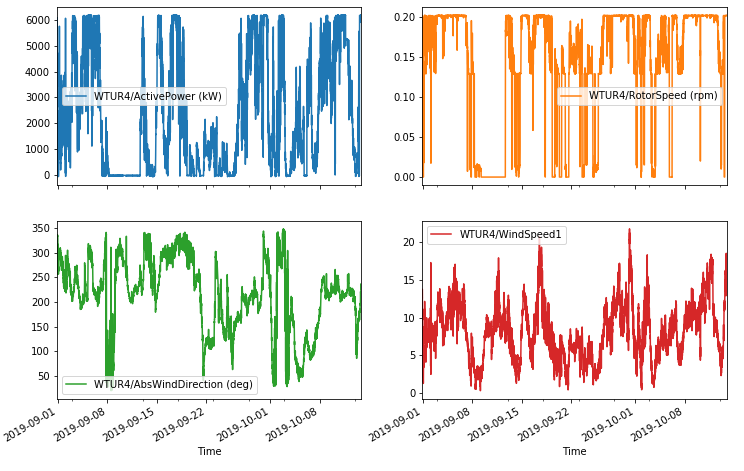
\includegraphics[width=0.6\textwidth]{data_exp/one_turbine_all_vals}
    \end{center}
    \caption{The data from one wind turbine} 
    \label{fig:data_one_wt}
\end{figure}

\section{Explained Varience of Principal Components}

One interesting point of comparison for the different wind turbines is the cumulative explained variance of a wind turbine for a given set of principal components. 
The total variance is the sum of the variences of the individual principal components. 
Since these multivariate time series have four dimensions four principle components should then be able to explain the variance of the entire dataset, as they are the eigenvectors of the covarience matrix of the time series. 
The explained variance of a principal component is the ration of the variance of said component to the total variance, and the cumulative explained variance of $n$ principal components is the sum of the explained variance of the $n$ first principal components. Since these turbines are in the same wind farm they are exposed to roughly the same environmental conditions, and one would expect them to have similar cumulative explained variance curves.

\begin{figure}[h]
    \begin{center}
    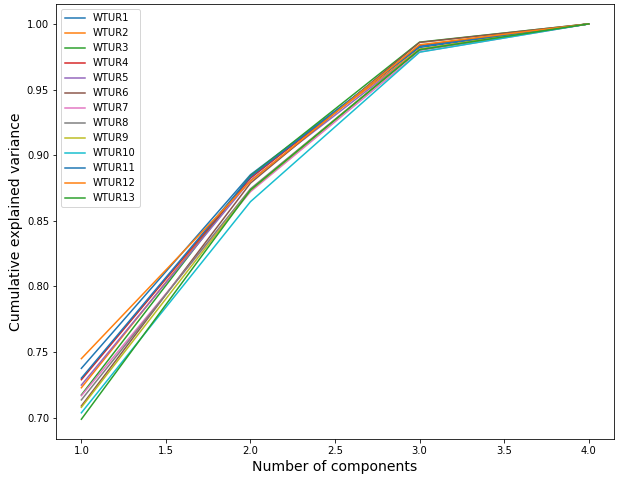
\includegraphics[width=0.5\textwidth]{data_exp/cumulative_explained_variance}
    \end{center}
    \caption{Cumulative explained variance for a given number of principal components} 
    \label{fig:cum_exp_var}
\end{figure}

In figure \ref{fig:cum_exp_var} there is a plot of the cumulative explained varience of the 13 turbines for a given set of principal components. 
As expected the total variance can be explained by four principle components for all wind turbines. 
However, as the number of principal components decreases there is a greater variety in the cumulutive explained variance for the different wind turbines. 
For only one principal component the biggest difference in cumulative explained varience is between turbine two at 75$\%$ explained variance, and turbine 13 at 70$\%$ explained variance.
This difference is not that substantial, from the plot in figure \ref{fig:cum_exp_var} one can see that all the curves follow more or less the same shape, so one cannot conclude that any of these curves are due to anomolous behaviour. \smallskip

\section{Reconstruction Error}

\begin{figure}[h]
    \begin{center}
    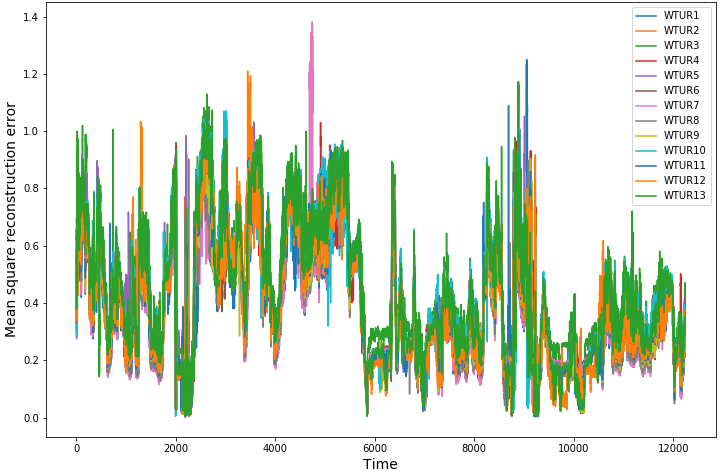
\includegraphics[width=0.5\textwidth]{data_exp/reconstruction_error}
    \end{center}
    \caption{Reconstruction error, when representing data with two principal components} 
    \label{fig:recon_error}
\end{figure}

Another indicator of anomolous behaviour is if the multivariate time series associated with a turbine has a significantly different $R_e$ compared to the multivariate time series of the other turbines in the wind farm. 
Figure \ref{fig:recon_error} shows the total MSE of the reconstructed time series associated with the different wind turbines. 
Here too, one can observe that the different wind turbines all follow approximately the same curve with regard to reconstruction error. 
With the exception of turbine seven has a slight spike at round about 5000 samples. 
To get a better reference of what constitutes anomolous behaviour, the data from one turbine will be artificially perturbed in the coming section. 

\section{Artificially Perturbation of Data}

\begin{figure}
    \begin{center}
    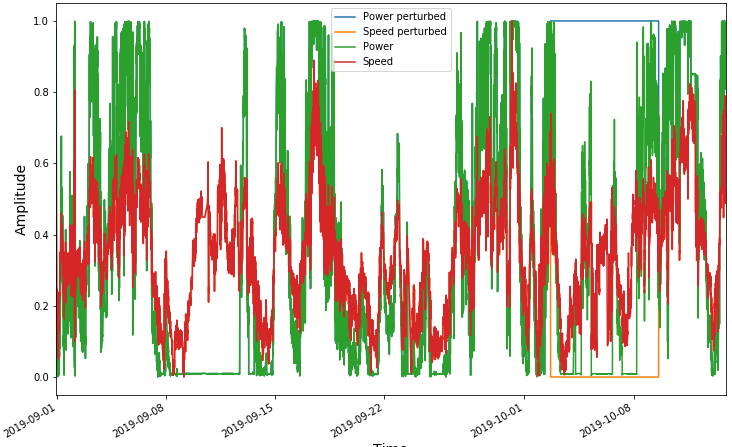
\includegraphics[width=0.5\textwidth]{data_exp/perturbed_vs_unperturbed}
    \end{center}
    \caption{Illustration of the perturbed data} 
    \label{fig:illu_perturbed_data}
\end{figure}

To artificially perturb the data 2000 samples from turbine 12 are changed. 
Sample 9000 to sample 1100 of the wind-speed and power time series are set to one and zero respectively.
Figure \ref{fig:illu_perturbed_data} illustrates this. 
This drastically changes the curve of cumulutive explained variance which is depicted in figure \ref{fig:cum_exp_var_pert}, and the reconstruction error of the time series associated with turbine 12 which is depicted in figure \ref{fig:recon_error_pert_vs_unpert} and \ref{fig:recon_error_pert}.
From figure \ref{fig:cum_exp_var_pert} one can see that the cumulative explained variance curve of turbine 12 is significantly lower than the curves of the other turbines in the farm, giving a reference of how some anomolous behaviour would show up in a cumulative explained variance curve. 
In figure \ref{fig:recon_error_pert_vs_unpert} one can see the reconstruction error of turbine 12 increases overall after the perturbation, and increases even more in the particular samples where the time series was altered. 
Finally, if one compares the reconstruction error of the perturbed data of wind turbine with the reconstruction error of the original data from the other turbines in figure \ref{fig:recon_error_pert}, one can see that the spike in turbine seven mentioned earlier is of the same magnitude as the spike in the reconstruction error of wind turbine 12 when artificially perturbed. 

\begin{figure}
    \begin{center}
    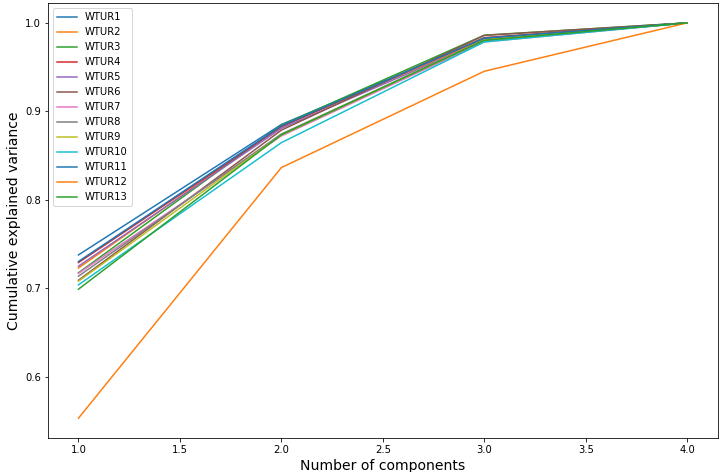
\includegraphics[width=0.5\textwidth]{data_exp/explained_variance_perturbed}
    \end{center}
    \caption{Cumulative explained variance for a given number of principal components with perturbed data} 
    \label{fig:cum_exp_var_pert}
\end{figure}

\begin{figure}
    \begin{center}
    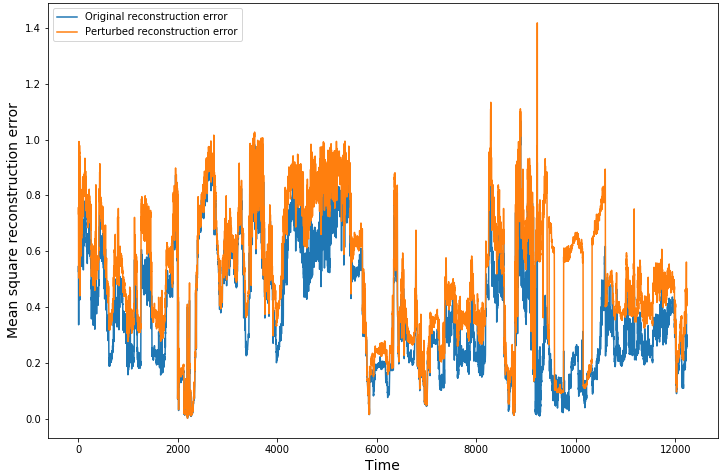
\includegraphics[width=0.5\textwidth]{data_exp/pert_vs_unpert_reconstruction_error}
    \end{center}
    \caption{Reconstruction of wind turbine 12 using two principal components, with original and perturbed data} 
    \label{fig:recon_error_pert_vs_unpert}
\end{figure}

\begin{figure}
    \begin{center}
    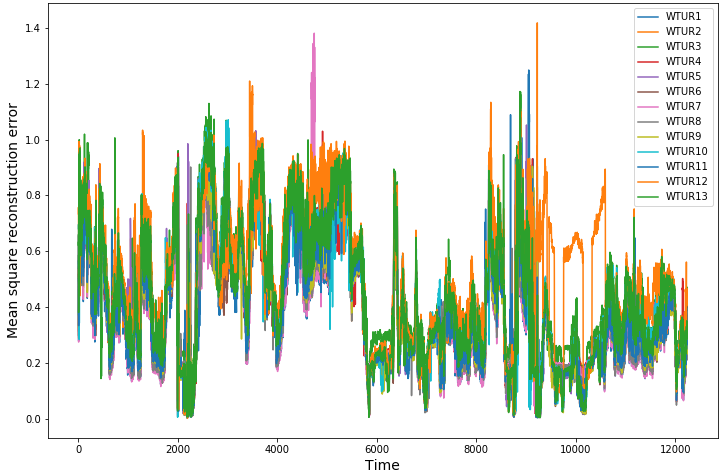
\includegraphics[width=0.5\textwidth]{data_exp/reconstruction_error_perturbed}
    \end{center}
    \caption{Reconstruction error, when representing data with two principal components using perturbed data} 
    \label{fig:recon_error_pert}
\end{figure}